\subsection{Die Konfiguration des \emph{Spawners}}

Die Konfiguration des \emph{Spawners} legt fest, wann und wo in der Simulation Züge erzeugt werden. Eine der Anforderungen an das System ist, dass der Benutzer in der Lage sein muss, diese Konfiguration durchzuführen. Weiterhin ist es wünschenswert, dass die Konfigurationen gespeichert werden können, um die zugehörigen Simulationen erneut oder in abgeänderter Form durchführen zu können. Zu Beginn des Projektes erbten die Klassen \code{Spawner}, \code{Schedule} und \code{ScheduleStrategy} von \code{BaseModel}. Somit ließen sich Instanzen dieser Klassen und ihrer Subklassen direkt in die Datenbank schreiben. Dieser Ansatz wurde jedoch verworfen, da das verwendete ORM \emph{peewee} nicht in der Lage ist, objektorientierte Vererbungshierachien ausreichend gut abzubilden. \emph{peewee} ordnet jeder Klasse eine Tabelle in der Datenbank zu. Es spielt dabei keine Rolle, ob es sich um eine abstrakte oder eine konkrete Klasse handelt. Ein \code{Schedule}-Objekt kann bspw. ein \code{RegularScheduleStrategy}-Objekt enthalten. Die Klasse \code{Schedule} hat jedoch nur Kenntnis von der abstrakten Klasse \code{ScheduleStrategy}. Die Abbildung durch \emph{peewee} erzeugt daher für die Tabelle \code{Schedule} lediglich einen Fremdschlüssel, der auf die ''abstrakte'' Tabelle \code{ScheduleStrategy} verweist. Referenzen auf abstrakte Klassen lassen sich also mit \emph{peewee} nicht abbilden.\\
\\
Wir haben uns stattdessen für die in \autoref{fig:spawner-config-class} dargestellte Architektur entschieden. Dem \code{Spawner} wird nun ein Konfigurationsobjekt (\code{SpawnerConfiguration}) zugewiesen. Über eine $m$:$n$-Beziehung, die durch die Klasse \code{SpawnerConfiguratioXSchedule} bereitgestellt wird, können einem \code{SpawnerConfiguration}-Objekt mehrere \code{ScheduleConfiguration}-Objekte zugewiesen werden, welches alle Informationen für ein \code{Schedule}-Objekt und ein dazugehöriges konkretes \code{ScheduleStrategy}-Objekt beinhaltet. Die Liste der anzufahrenden Haltestellen wird über die Klasse \code{ScheduleConfigurationXSimulationPlatform} referenziert. Über das Attribut \code{index} kann die Reihenfolge der Haltestellen abgebildet werden. Bei diesem Vorgehen ist zu beachten, dass die $m$:$n$-Beziehungen aus der Datenbank nicht vor dem Programmierer versteckt wurden. Stattdessen wurden sie 1:1 in das objektorientierte Paradigma übernommen. Weiterhin gibt es keine Subklassen von \code{Scheduke} und \code{ScheduleStrategy} mehr. Sämtliche Attribute der Subklassen finden sich in \code{ScheduleConfiguration} wieder. Entsprechend wird stets nur eine Teilmenge dieser Attribute verwendet. Um die Subklassen dennoch abzubilden, existieren die Felder \code{schedule\_type} und \code{strategy\_type}. Das hier beschriebene Problem wurde bei der Auswahl des ORM nicht vorhergesehen. Um allerdings nicht eion neues ORM in das System integrieren zu müssen, haben wir uns für diese Lösung entschieden. Sie bot einen Zeitvorteil und funktionierte ausreichend gut.

\begin{figure}[!ht]
	\centering
	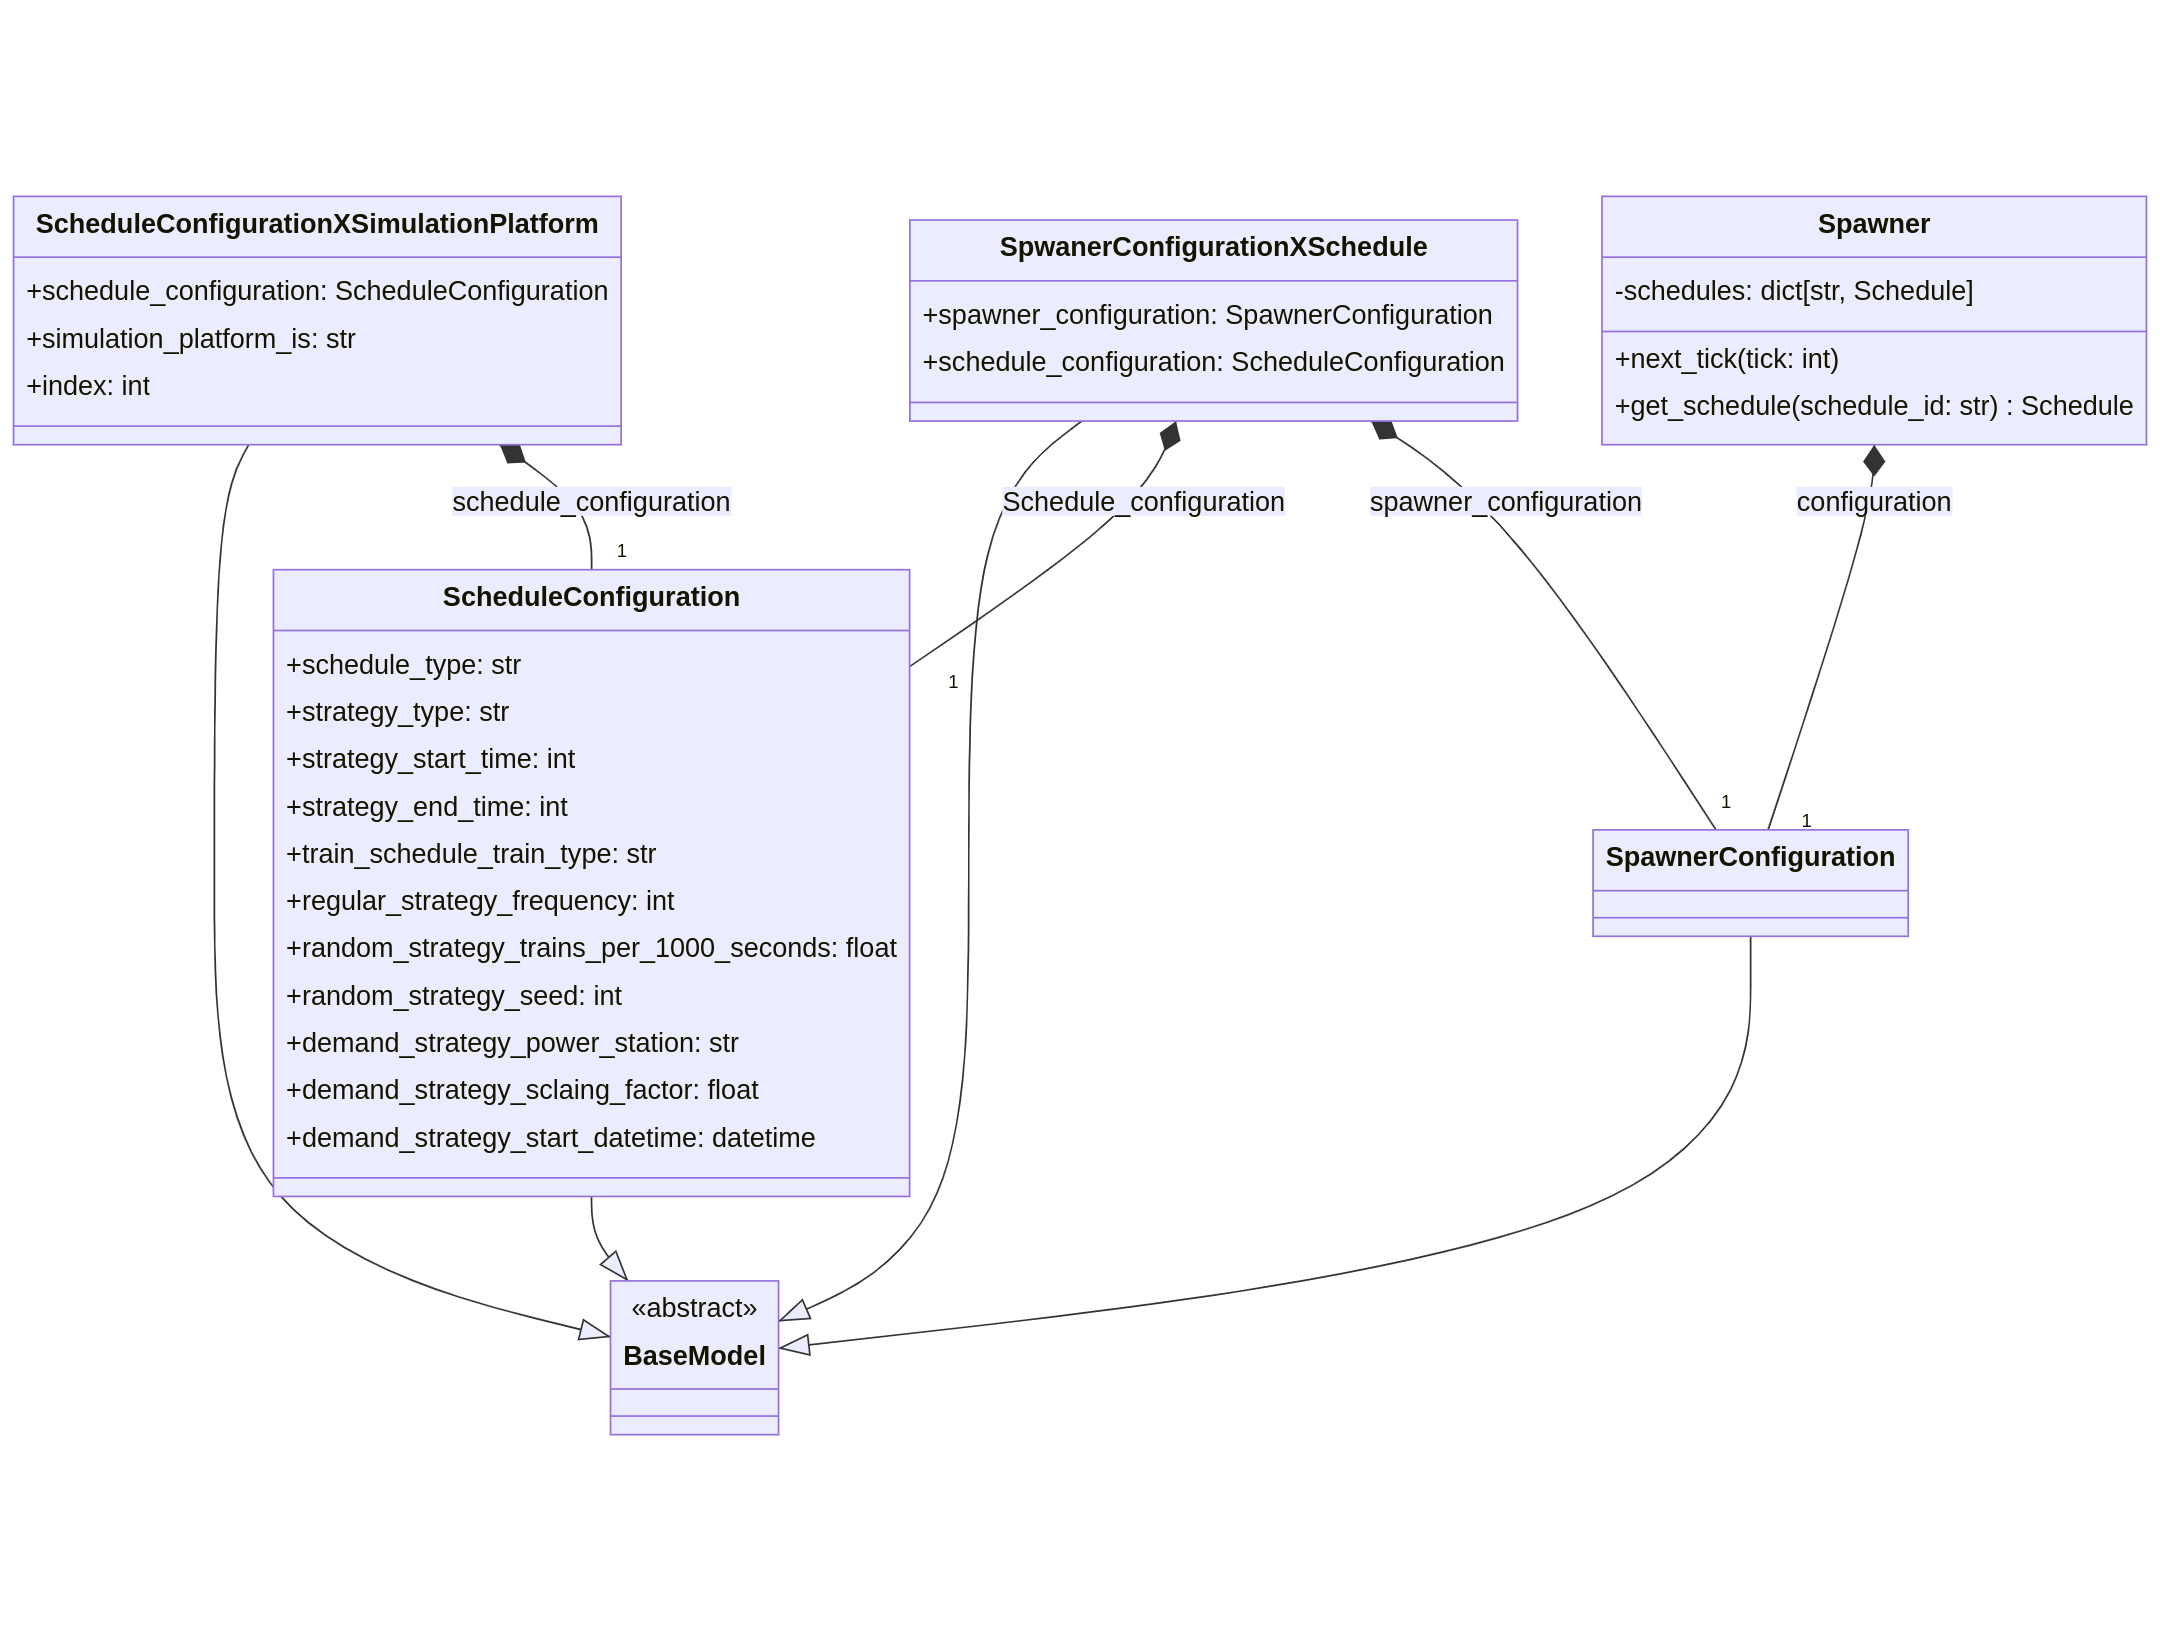
\includegraphics[width=1.0\linewidth]{images/diagrams/spawner-config-class.png}
	\caption{Klassendiagramm der \emph{Spawner}-Konfiguration}
	\label{fig:spawner-config-class}
\end{figure}

Alle zur Konfiguration gehörenden Klassen werden in JSON-serialisierter Form vom Benutzer über die \emph{REST-API} übertragen \cite{kamp_architektur_2023}. Sie werden daraufhin deserialisiert und in der Datenbank abgelegt. Aus diesen Kofigurationsobjekten können dann ein \code{Spawner}, \code{Schedule}-Objekte und \code{ScheduleStrategy}-Objekte erzeugt werden. Dafür wurde das Entwurfsmuster der \emph{Factory-Method} verwendet. \autoref{fig:spawner-factory-class} zeigt, dass die Klassen \code{Schedule} und \code{ScheduleStrategy} bzw. ihre Subklassen ihre eigenen \emph{Factories} sind. Sie besitzen zu diesem Zweck jeweils eine \emph{Klassen}-Methode \code{from\_schedule\_configuration}, welche als \emph{Factory-Method} fungiert.

\begin{figure}[!ht]
	\centering
	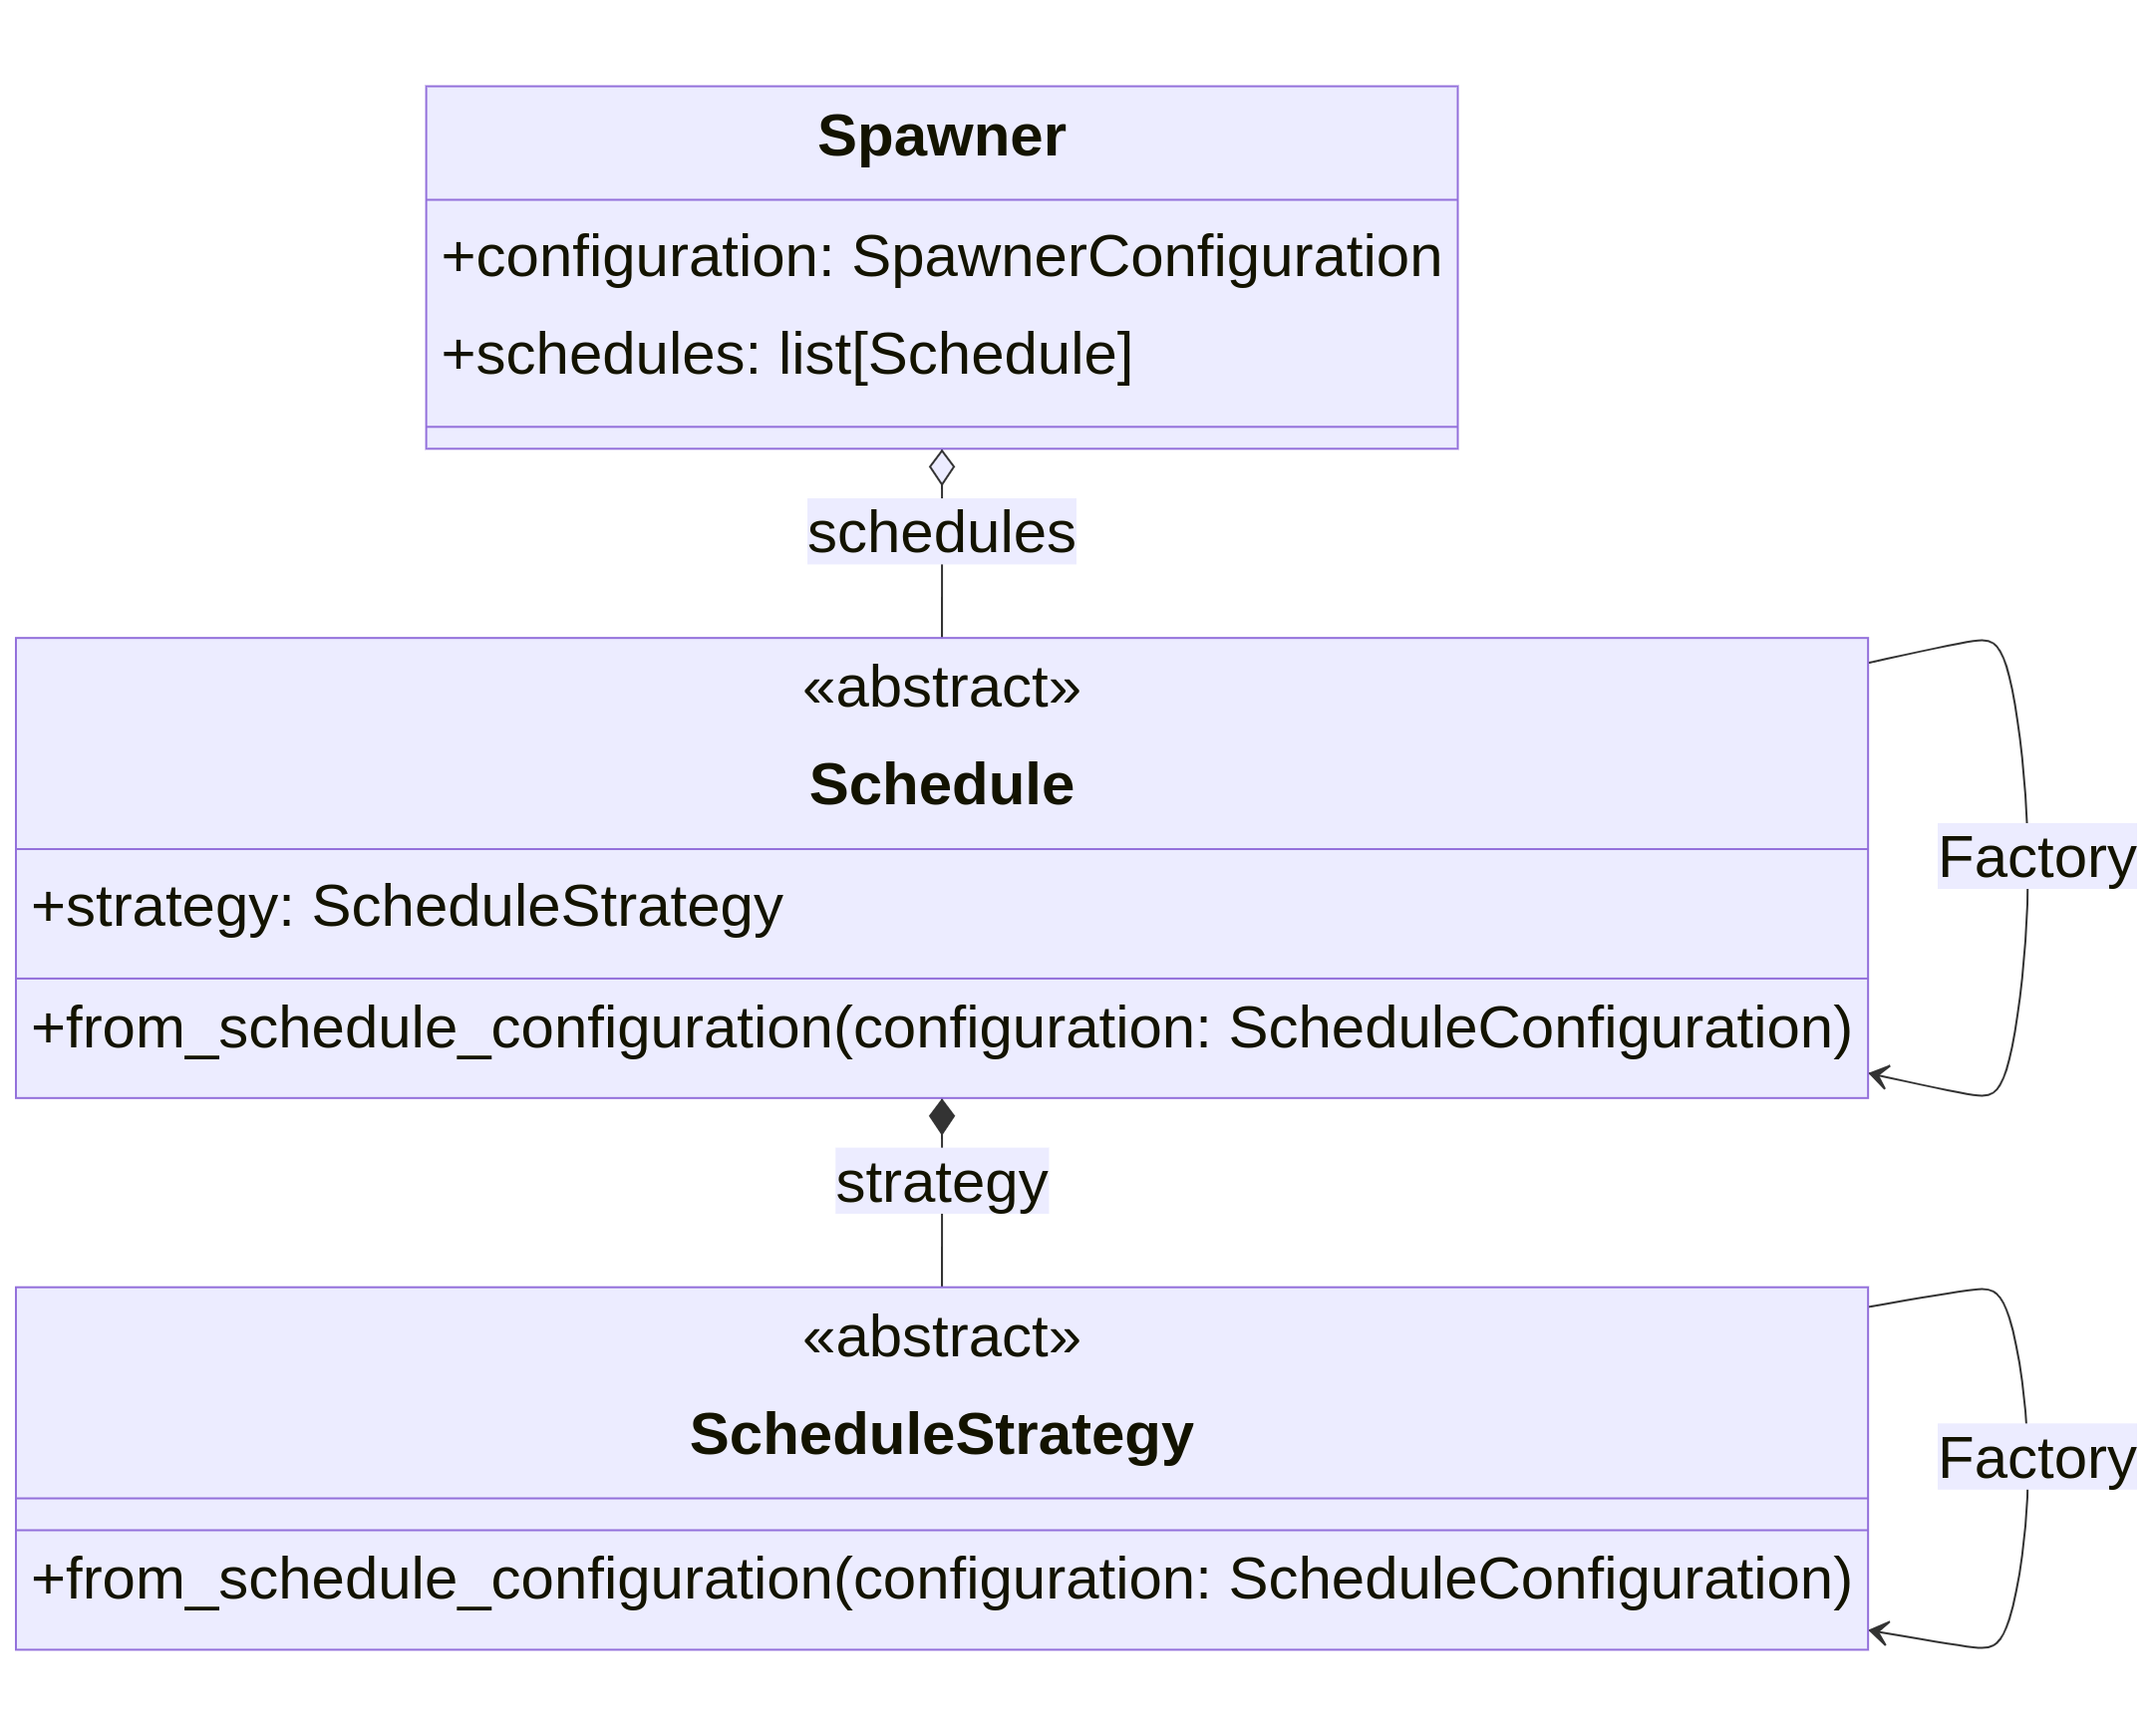
\includegraphics[width=1.0\linewidth]{images/diagrams/spawner-factory-class.png}
	\caption{Klassendiagramm der \emph{Spawner}-Konstruktion}
	\label{fig:spawner-factory-class}
\end{figure}

\autoref{fig:spawner-factory-seq} zeigt, wie aus einer Konfiguration, entsprechende Objekte erzeugt werden. Das \code{Spawner}-Objekt ruft für jedes referenzierte \code{ScheduleConfiguration}-Objekt die \emph{Factory-Method} der Klasse \code{Schedule} auf (1). Diese instanziiert daraufhin ein dem Wert des Attributes \code{ScheduleType} entsprechendes \code{Schedule}-Objekt und ein \code{ScheduleStrategy}-Objekt durch Aufruf der \emph{Factory-Method} der Klasse \code{ScheduleStrategy} und erneute Übergabe des Konfigurationsobjektes (2). Beide \emph{Factory-Methods} lesen die benötigten Werte für die Attribute der zu erzeugenden Objekte aus dem Konfigurationsobjekt und geben dann das fertige Objekt zurück. Jedes \code{Schedule}-Objekt kann dass das erzeugte \code{ScheduleStrategy}-Objekt im Attribut \code{strategy} speichern. Das \code{Spawner}-Objekt kann die erzeugten \code{Schedule}-Objekte in der Liste \code{schedules} speichern.

\begin{figure}[!ht]
	\centering
	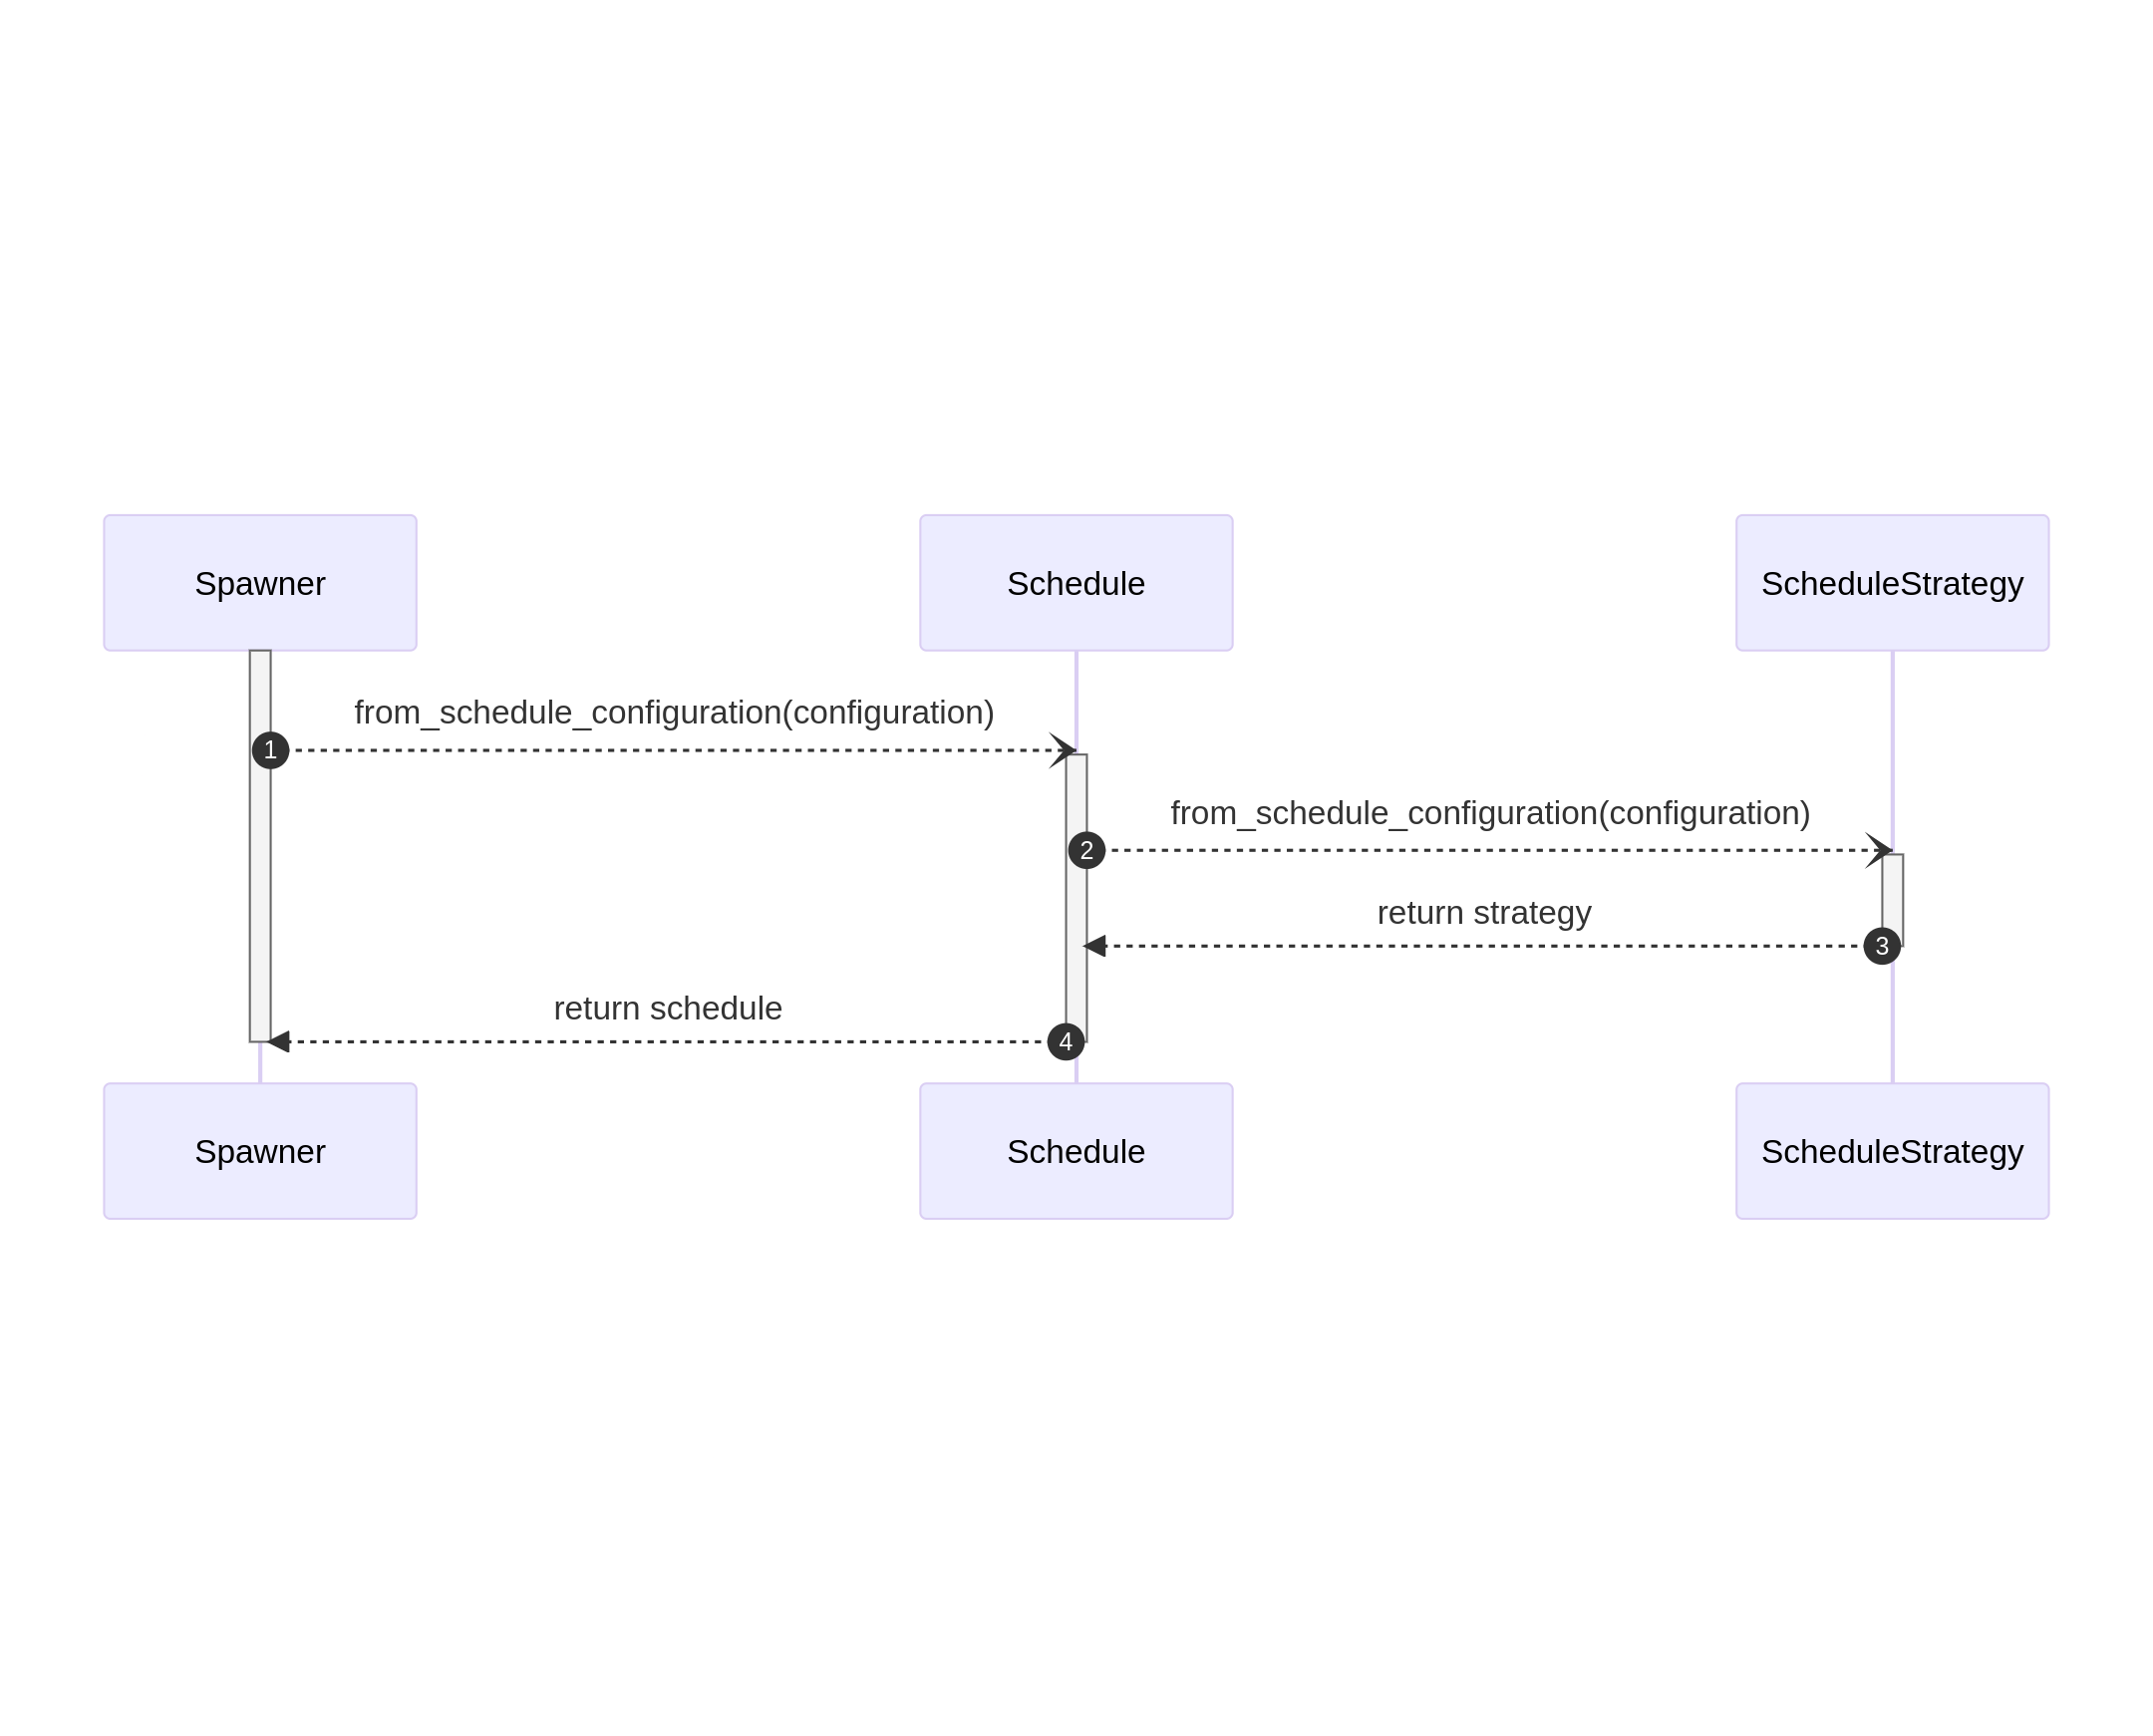
\includegraphics[width=1.0\linewidth]{images/diagrams/spawner-factory-seq.png}
	\caption{Sequenzdiagramm der \emph{Spawner}-Konstruktion}
	\label{fig:spawner-factory-seq}
\end{figure}
